\documentclass{article}
\usepackage[dblblindworkshop]{neurips_2026}
\workshoptitle{Physical Understanding and Dynamics Modeling}

\usepackage[utf8]{inputenc}
\usepackage[T1]{fontenc}
\usepackage{hyperref}
\usepackage{url}
\usepackage{booktabs}
\usepackage{amsmath,amsfonts}
\usepackage{microtype}
\usepackage{xcolor}
\usepackage{graphicx}
\usepackage{subcaption}
\usepackage{multirow}
\setcitestyle{numbers}

\title{PhysWM: Grounding Predictive World Models in Physical Equations}
\author{Anonymous Authors}

\newcommand{\model}{\textsc{PhysWM}}
\newcommand{\patha}{\hat{s}^{A}_{t+1}}
\newcommand{\pathb}{\hat{s}^{B}_{t+1}}

\begin{document}
\maketitle

\begin{abstract}
Predictive world models can forecast dynamics without organizing their representations around the physical variables governing a system. We introduce \model, a two-path architecture that grounds an action-conditioned predictive world model through known physical equations. A neural path predicts the next state from data, while an equation path maps the same predictive latent through a low-capacity probe to physical variables and a frozen differentiable solver. Without parameter labels, the equation path learns to reproduce the neural path's stopped-gradient prediction. We evaluate grounding through prediction, semantic readout, parameter substitution, and multi-horizon equation rollouts. On PokeWorld, the predictor beats persistence and inferred variables reduce seven-step rollout error relative to shuffled variables across three seeds. On randomized PushT, inferred effective dynamics beat shuffled episode assignments in all three seeds. The results support equation-compatible effective coordinates while exposing limits from non-identifiability and simulator mismatch.
\end{abstract}

\section{Introduction}

World models compress observations and actions into representations useful for predicting future dynamics. Predictive accuracy alone, however, does not ensure that these representations expose mass, damping, stiffness, friction, or control response. A high-capacity predictor may exploit trajectory correlations while leaving the governing physical factors entangled. This separates predicting \emph{what happens} from representing \emph{why the system evolves that way}.

We study whether known physical equations can ground a flexible predictive world model without physical-parameter annotations. \model produces two next-state predictions from the same action-conditioned latent (Fig.~\ref{fig:method}). Path A is a learned decoder trained on observed transitions. Path B maps the latent to a compact vector $\hat\theta$ and evaluates a frozen differentiable solver. Crucially, Path B targets Path A's stopped-gradient prediction rather than the dataset state directly. The neural path remains anchored to data and free to absorb model mismatch; the physical path asks whether the model's predictive belief admits a compact equation-based explanation.

Our contribution is threefold. First, we introduce a shared-latent, two-path objective for grounding predictions in a supplied equation family without parameter labels. Second, we evaluate grounding functionally by changing only the solver's parameter vector while holding states, actions, weights, and equations fixed. Third, we distinguish \emph{semantic parameters}, which match named ground-truth quantities, from \emph{effective physical coordinates}, which improve equation rollouts but may compensate for non-identifiability or solver mismatch.

\begin{figure}[t]
  \centering
  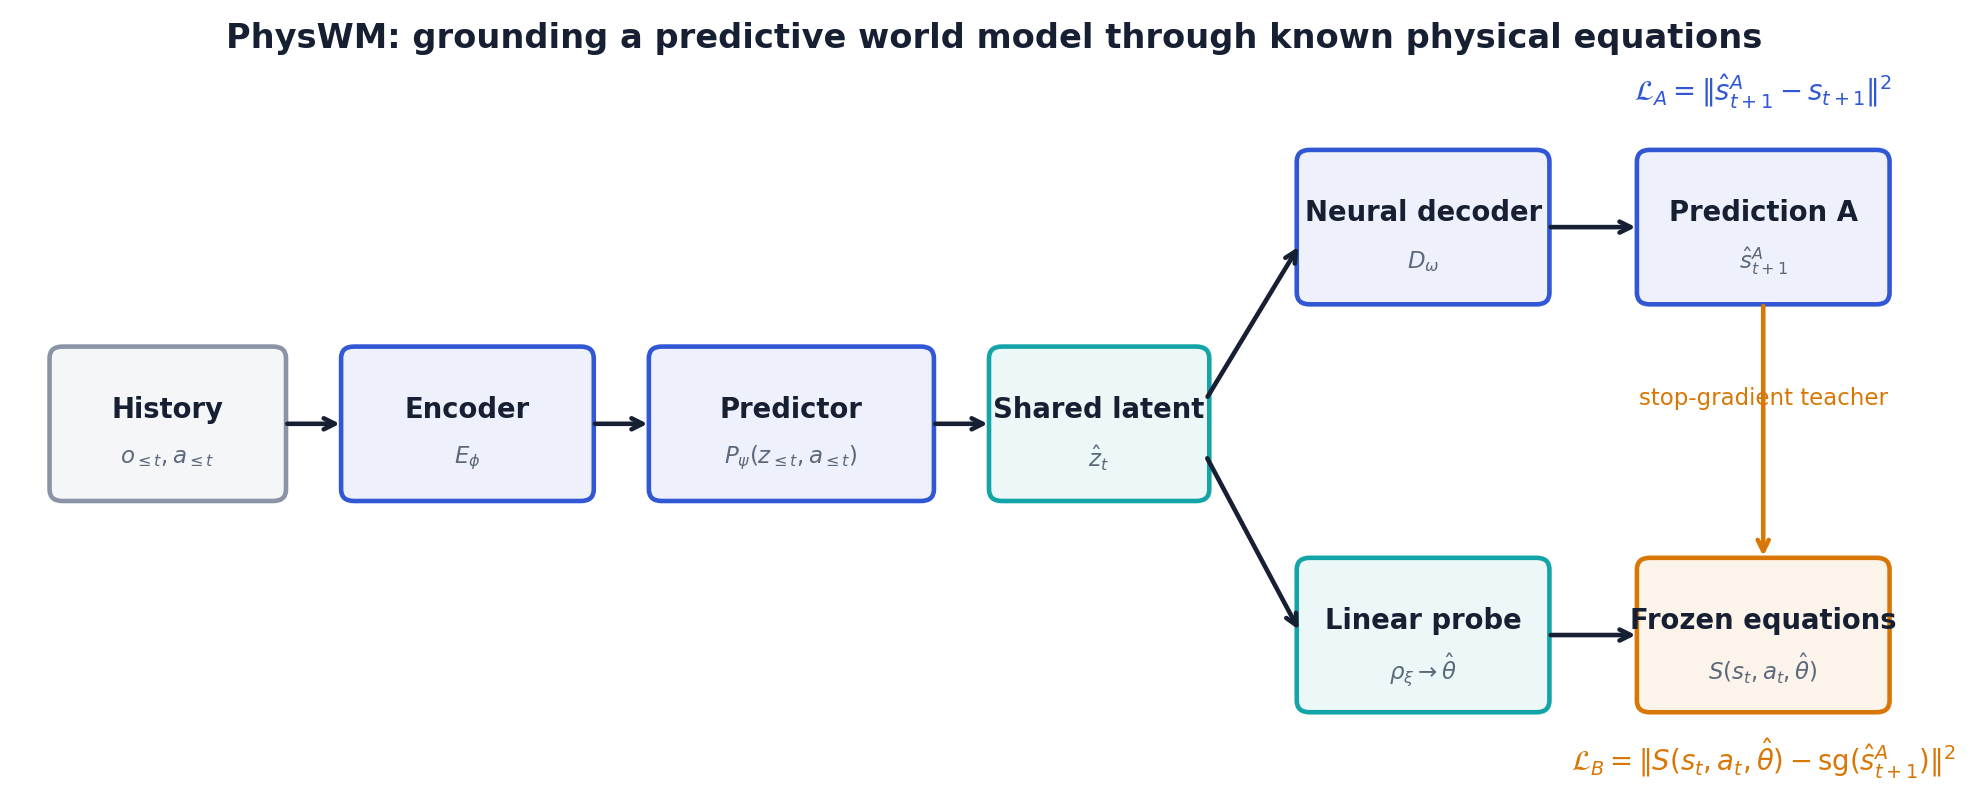
\includegraphics[width=\linewidth]{../generated/fig1_architecture.png}
  \caption{\model grounds a learned predictor through known equations. Both paths read the same action-conditioned latent. Path A is supervised by the observed next state; Path B explains Path A's stopped-gradient prediction through a compact physical vector and a frozen differentiable solver.}
  \label{fig:method}
\end{figure}

\section{Equation-grounded predictive representations}

Given observations $o_t$, actions $a_t$, and prediction state $s_t$, an encoder and causal action-conditioned predictor form
\begin{equation}
z_t=E_\phi(o_t), \qquad \hat z_t=P_\psi(z_{\leq t},a_{\leq t}).
\end{equation}
The neural decoder produces $\patha=D_\omega(\hat z_t)$ and is trained in normalized state space:
\begin{equation}
\mathcal L_A=\|N(\patha)-N(s_{t+1})\|_2^2.
\end{equation}
A bounded low-capacity probe pools only causal context latents,
\begin{equation}
\hat\theta=\operatorname{Bound}\!\left(\rho_\xi(\operatorname{Pool}(\{\hat z_t\}_{t\in\mathcal C}))\right),
\end{equation}
and a frozen solver $S$, containing no learnable parameters, produces $\pathb=S(s_t,a_t,\hat\theta)$. The grounding loss is
\begin{equation}
\mathcal L_B=\|N(\pathb)-\operatorname{sg}(N(\patha))\|_2^2,
\qquad \mathcal L=\mathcal L_A+\alpha\mathcal L_B.
\end{equation}
The stopped target prevents $\mathcal L_B$ from moving the Path-A decoder through its target edge, while gradients through $S$, $\rho_\xi$, and $P_\psi$ shape the shared predictor. The default probe is linear, preventing it from hiding another world model. $\hat\theta$ is always a forward-pass output, never a free test-time optimization variable.

\paragraph{Causal evaluation split.} The identifier observes only completed context transitions. Metrics are computed on later query transitions, and no query outcome is accessible to the probe. With the default eight-frame window, four completed transitions form the context. Functional evaluation uses eight context transitions followed by seven held-out rollout transitions.

\paragraph{Grounding criterion.} We call a coordinate physically grounded when reading it from the predictive latent allows the fixed equations to explain held-out dynamics better than a coordinate carrying no episode-specific information. This is deliberately weaker than claiming recovery of a unique material parameter: trajectories may identify only ratios such as stiffness/mass, and approximate solvers may induce compensating effective values.

\section{Evaluation}

We test four complementary properties. (1) \emph{Predictive adequacy}: Path A must beat persistence, $\hat s_{t+1}=s_t$. (2) \emph{Semantic readout}: where labels exist, a supervised linear probe measures held-out episode-level $R^2$. (3) \emph{Parameter substitution}: the solver receives the inferred vector, another episode's shuffled vector, nominal constants, or true parameters when available. (4) \emph{Multi-horizon rollout}: the same substitutions are rolled forward under fixed held-out actions. All errors are scaled per state dimension.

\paragraph{PokeWorld.} This synthetic contact benchmark varies mass, contact stiffness, and drag while keeping object appearance fixed. Its differentiable solver matches the generator, providing true-parameter and solver-adequacy certificates. The reported runs use 2,048 episodes, a tiny CNN diagnostic encoder, and three seeds.

\paragraph{Randomized PushT.} This planar manipulation benchmark varies effective dynamics. Its solver is approximate and ground-truth labels are unavailable for most coordinates, making inferred-versus-shuffled substitution the primary test. The reported runs use 512 episodes and three seeds.

\begin{table}[t]
\centering
\caption{Mean $\pm$ sample standard deviation over three seeds. RMSE is lower better; $R^2$ is higher better.}
\label{tab:main}
\small
\setlength{\tabcolsep}{4pt}
\begin{tabular}{llcc}
\toprule
Benchmark & Metric & Baseline / control & \model{} \\
\midrule
PokeWorld & Query prediction RMSE & Persistence $0.383\pm0.052$ & $0.282\pm0.046$ \\
PokeWorld & Stiffness $R^2$ & Predictive $0.754\pm0.017$ & $0.784\pm0.029$ \\
PokeWorld & Mass $R^2$ & Predictive $0.241\pm0.028$ & $0.237\pm0.055$ \\
PokeWorld & Drag $R^2$ & Predictive $-0.191\pm0.052$ & $-0.146\pm0.043$ \\
PokeWorld & 7-step solver RMSE & Shuffled $0.220\pm0.018$ & Inferred $0.193\pm0.010$ \\
PushT & Solver substitution RMSE & Shuffled $0.267\pm0.013$ & Inferred $0.208\pm0.011$ \\
\bottomrule
\end{tabular}
\end{table}

\section{Results and discussion}

\paragraph{Accurate prediction is not uniform parameter recovery.} On PokeWorld, Path A beats persistence in every seed (Table~\ref{tab:main}). Stiffness is strongly linearly readable and improves modestly under equation grounding. Mass remains weak, and drag has negative held-out $R^2$ for both models. Thus the results do not support uniform recovery of named parameters. They instead expose an observability boundary: an equation-compatible representation can be useful even when individual semantic factors are not uniquely recoverable.

\begin{figure}[t]
  \centering
  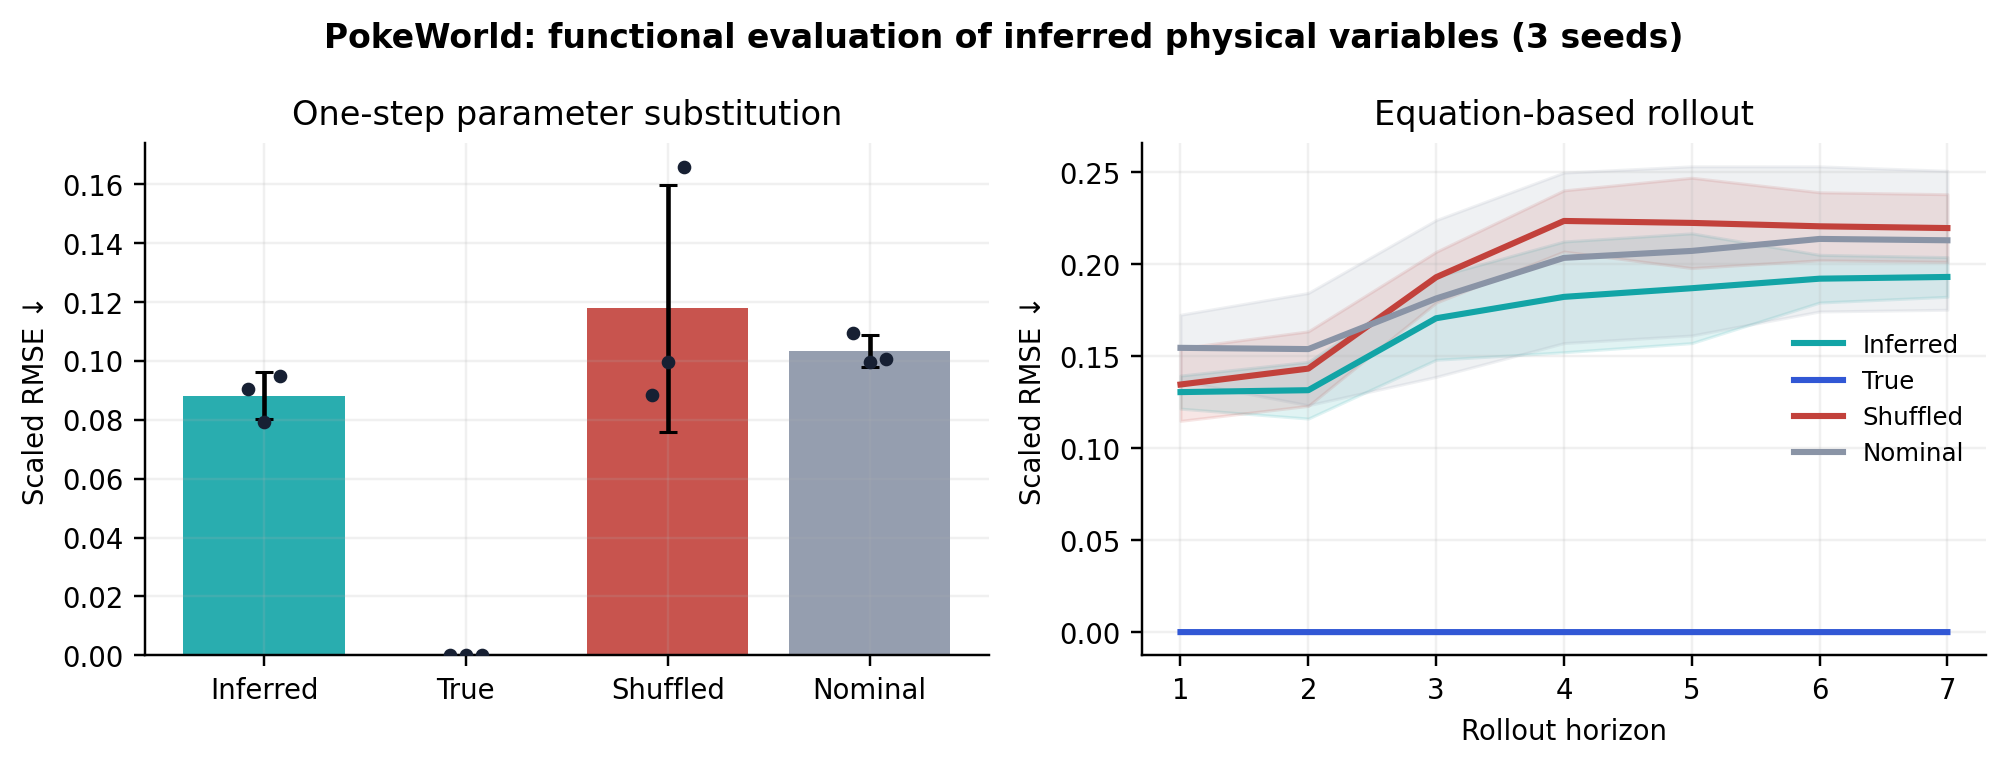
\includegraphics[width=\linewidth]{../generated/fig2_pokeworld_functional.png}
  \caption{PokeWorld functional evaluation. Left: one-step error after substituting inferred, true, shuffled, or nominal parameters. Right: equation-rollout error over horizon. Curves and error bars show mean and sample standard deviation over three seeds.}
  \label{fig:poke}
\end{figure}

\paragraph{Inferred coordinates improve equation rollouts.} In PokeWorld one-step evaluation, inferred coordinates achieve $0.088\pm0.008$ scaled RMSE versus $0.118\pm0.042$ for shuffled and $0.103\pm0.006$ for nominal values. The one-step ordering is not uniform across seeds. At seven steps, however, inferred coordinates beat shuffled assignments in every seed, yielding $0.193\pm0.010$ versus $0.220\pm0.018$ (Fig.~\ref{fig:poke}). True parameters are nearly exact because the solver matches the generator.

On PushT, inferred variables obtain $0.208\pm0.011$ substitution RMSE versus $0.267\pm0.013$ for shuffled assignments. Inferred values beat shuffled in all three seeds and nominal values in two of three. Solver sensitivity is concentrated in the agent's proportional and derivative gains, so this supports episode-specific effective control dynamics rather than complete contact-parameter identification. Moreover, Path A fails to beat persistence in one PushT seed, limiting the cross-benchmark claim.

\paragraph{Simulator mismatch changes the meaning of $\hat\theta$.} A corrected FetchPush diagnostic illustrates the risk. After fixing a 10$\times$ gripper-integration error, inferred variables still outperform true mass and friction by a large margin, while solver-space task success is identical for every parameter source. The probe is therefore compensating for residual equation mismatch. This motivates reporting solver adequacy and sensitivity alongside parameter accuracy and describing $\hat\theta$ as an effective physical coordinate unless semantic identifiability is independently certified.

\section{Conclusion and limitations}

\model grounds a predictive world model by requiring its shared action-conditioned representation to support a compact explanation through known physical equations. Current results show improved equation-based rollouts relative to shuffled episode variables, especially over longer horizons, but not uniform recovery of named parameters. The supplied equations, observation process, and solver fidelity determine what can be identified.

The study is limited to diagnostic tiny-CNN experiments on two usable multi-seed benchmarks. It does not discover equations, select informative actions, or demonstrate closed-loop planning or sim-to-real transfer. Corrected FetchPush and stable CartPole experiments remain incomplete, and pretrained visual encoders require paper-scale evaluation. These limitations define the next step: test whether equation grounding remains beneficial with strong visual backbones and whether uncertainty-aware actions can actively reveal otherwise ambiguous physical coordinates.

\begin{thebibliography}{9}
\bibitem{gradsim} M. Murthy et al. gradSim: Differentiable simulation for system identification and visuomotor control. \emph{ICLR}, 2021.
\bibitem{piwm} Physically Interpretable World Models via Weakly Supervised Representation Learning. arXiv:2412.12870, 2024.
\bibitem{ldr} Learning How the World Evolves: Extrapolative Video World Models via Latent Dynamics Reasoning. arXiv:2608.09926, 2026.
\bibitem{phylatent} PhyLatent: Learning Dynamics-Relevant Representations for JEPA World Models. arXiv:2608.05720, 2026.
\bibitem{invisible} The Invisible Hand of Physics: When Video Diffusion Models Know More Than They Show. arXiv:2606.05328, 2026.
\end{thebibliography}

\end{document}
